\begin{pastexam}[label={px:ccu-111-swa-08}]{中正資工所甲組 111 學年度 第 16 題}
（單選）

(4\%) To find the articulation points in the graph below, start with constructing a depth-first
spanning tree by doing a depth-first search of the graph. Instead of choosing an arbitrary vertex
to start, your first vertex must be set to vertex B, and select the smallest vertex in alphabetical
order first when performing the depth-first search. The depth-first number starts at 1.
\begin{center}
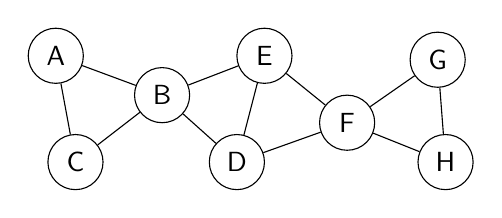
\begin{tikzpicture}[every node/.style={circle,draw,minimum size=7mm,inner sep=0pt,font=\sffamily}]
\node (A) at (0,1.1) {A}; \node (B) at (1.35,0.6) {B}; \node (C) at (0.25,-0.25) {C};
\node (E) at (2.65,1.1) {E}; \node (D) at (2.3,-0.25) {D}; \node (F) at (3.7,0.25) {F};
\node (G) at (4.85,1.05) {G}; \node (H) at (4.95,-0.25) {H};
\draw (A)--(B) (A)--(C) (C)--(B) (B)--(E) (B)--(D) (E)--(D) (E)--(F) (D)--(F) (F)--(G) (F)--(H) (G)--(H);
\end{tikzpicture}
\end{center}

16.1 (1\%) (\quad) What are the edges of the depth-first spanning tree?

\quad a.~(A, B), (A, C), (B, E), (B, D), (D, F), (F, G), (F, H)\\
\quad b.~(B, C), (A, C), (B, D), (D, F), (E, F), (F, G), (G, H)\\
\quad c.~(A, B), (B, C), (B, E), (B, D), (D, F), (F, G), (F, H)\\
\quad d.~(A, B), (A, C), (B, D), (D, E), (E, F), (F, G), (G, H) \qquad e.~None of the above

16.2 (2\%) (\quad) What are the output value of the low function (i.e., $\mathit{low}(v)$) for each
vertex (in the order of A, B, C, D, E, F, G, H).

\quad a.~(1, 2, 1, 1, 1, 1, 7, 6) \qquad b.~(1, 1, 1, 1, 1, 4, 6, 6) \qquad c.~(1, 1, 1, 1, 1, 1, 6, 6)\\
\quad d.~(1, 1, 1, 1, 1, 6, 6, 6) \qquad e.~(1, 1, 1, 4, 5, 6, 6, 6) \qquad f.~None of the above

16.3 (1\%) (\quad) What are the articulation points in the graph?

\quad a.~(B, F) \qquad b.~(B, F, G) \qquad c.~(A, D, F) \qquad d.~(B, G) \qquad e.~None of the above
\end{pastexam}

\begin{pastsoln}
答案：16.1 選 d，16.2 選 b，16.3 選 a。

做法照資結書第~23.5~節。 圖的鄰接（依字母排）：
A：B, C；\ B：A, C, D, E；\ C：A, B；\ D：B, E, F；\ E：B, D, F；\ F：D, E, G, H；\ G：F, H；\ H：F, G。

\textbf{16.1 DFS 樹。} 從 B 出發，每次走字母最小的未拜訪鄰點，括號裡是 DFS 編號 $d$：
\begin{enumerate}
\item B(1) 的鄰點 A 最小，走到 A(2)。
\item A 的鄰點 B 已拜訪，走 C(3)。 C 的鄰點 A、B 都拜訪過（C--B 是後向邊），C 結束，退回 A，A 結束，
退回 B。
\item B 的下一個未拜訪鄰點是 D，走到 D(4)；D 的鄰點 B 已拜訪，走 E(5)。
\item E 的鄰點 B 已拜訪（E--B 是後向邊）、D 是父節點，走 F(6)。
\item F 的鄰點 D 已拜訪（F--D 是後向邊）、E 是父節點，走 G(7)；G 的鄰點 F 是父節點，走 H(8)。
H 的鄰點 F 已拜訪（H--F 是後向邊），結束，一路退回 B。
\end{enumerate}
樹邊是 (B, A)、(A, C)、(B, D)、(D, E)、(E, F)、(F, G)、(G, H)，和 d 相同（無向邊不分順序）。 其他選項：
a 有 (B, E)、(F, H)，但 E 是從 D 走到的，H 是從 G 走到的；b 有 (B, C)，但 C 是從 A 走到的；c 同樣有
(B, C)、(B, E)。 後向邊是 C--B、E--B、F--D、H--F。

\textbf{16.2 low 值。} 照資結書第~23.5~節的定義，$\mathit{low}[u]$ 取 $d[u]$、子節點的 $\mathit{low}$、
$u$ 的後向邊另一端的 $d$ 三者的最小值。 從 DFS 樹的葉子往上算：
\begin{center}
\begin{tabular}{cccl}
\toprule
頂點 & $d$ & 後向邊到 & $\mathit{low}$ \\
\midrule
H & 8 & F（6） & $\min(8, 6) = 6$ \\
G & 7 & --- & $\min(7, \mathit{low}[H] = 6) = 6$ \\
F & 6 & D（4） & $\min(6, 4, \mathit{low}[G] = 6) = 4$ \\
E & 5 & B（1） & $\min(5, 1, \mathit{low}[F] = 4) = 1$ \\
D & 4 & --- & $\min(4, \mathit{low}[E] = 1) = 1$ \\
C & 3 & B（1） & $\min(3, 1) = 1$ \\
A & 2 & --- & $\min(2, \mathit{low}[C] = 1) = 1$ \\
B & 1 & --- & $1$ \\
\bottomrule
\end{tabular}
\end{center}
依 A, B, \ldots, H 的順序是 $(1, 1, 1, 1, 1, 4, 6, 6)$，選 b。 其他選項：a 的 $\mathit{low}[B] = 2$ 不可能（$\mathit{low}$
不超過自己的 $d = 1$），$\mathit{low}[G] = 7$ 漏了子節點 H 的 $6$；c 把 $\mathit{low}[F]$ 算成 $1$，F 的子樹裡沒有
後向邊回到 B；d 把 $\mathit{low}[F]$ 算成 $6$，漏了後向邊 F--D；e 的 D、E 漏了後向邊 E--B。

\textbf{16.3 割點。} 用資結書定理~23.8 和定理~23.9：
\begin{itemize}
\item 根 B 在 DFS 樹裡有 A、D 兩個子節點，是割點。
\item A：子節點 C 的 $\mathit{low} = 1 < d[A] = 2$，不是。
\item D：子節點 E 的 $\mathit{low} = 1 < 4$，不是；E：子節點 F 的 $\mathit{low} = 4 < 5$，不是。
\item F：子節點 G 的 $\mathit{low} = 6 \ge d[F] = 6$，是割點。
\item G：子節點 H 的 $\mathit{low} = 6 < 7$，不是。 C、H 是葉子，不是。
\end{itemize}
割點是 B、F，選 a。 直接看圖也對得上：拿掉 B，$\{A, C\}$ 和其他頂點分開；拿掉 F，$\{G, H\}$ 分開。
b、d 的 G 拿掉後 F、H 還有邊相連，不是割點；c 的 A、D 也不是。
\end{pastsoln}
